%introduction-example


\usebackgroundtemplate{%             declare it
\tikz[overlay,remember picture] \node[opacity=1, at=(current page.center)] {
   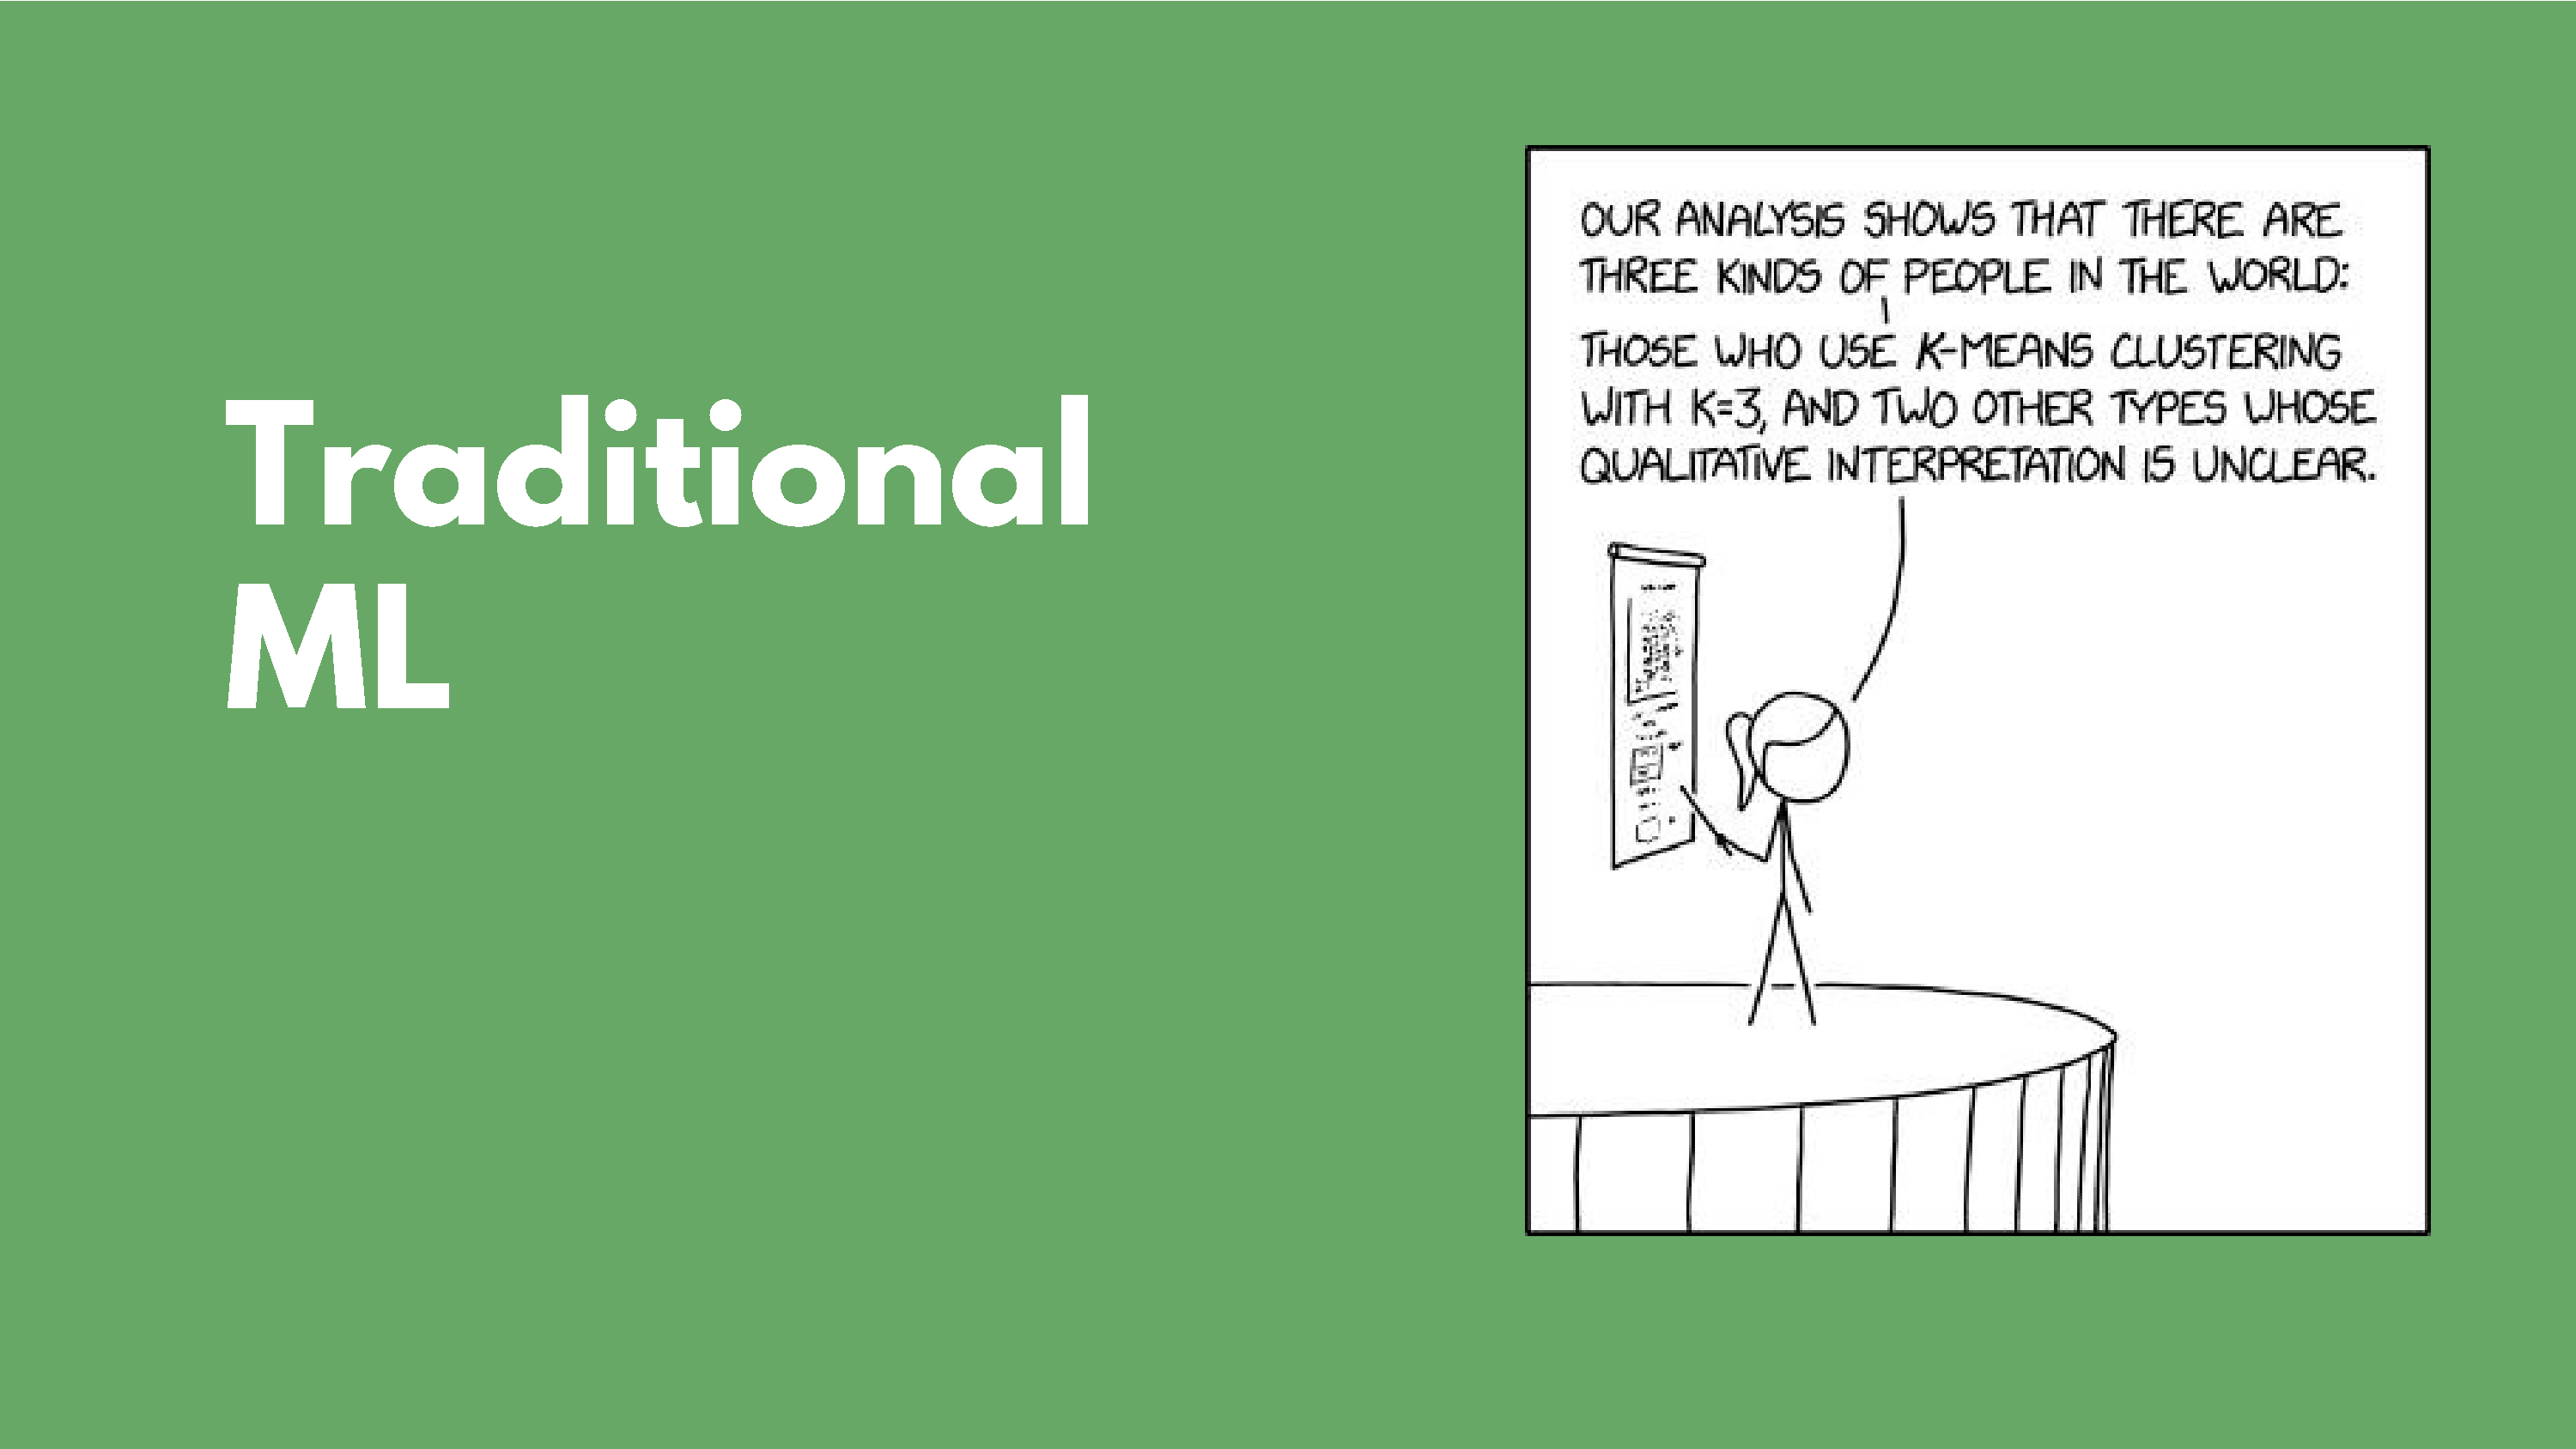
\includegraphics[height=\paperheight,width=\paperwidth]{images/tradML.pdf}};
}

\begin{frame}
\end{frame}

\usebackgroundtemplate{ }
%edit as needed



\begin{frame}{Traditional Machine learning}
The older/traditional way of applying machine learning consisted of the following steps:
    \begin{enumerate}[$\bullet$]
        \item \textbf{Feature Extraction}: Features which can be used to discriminate between classes is captured. This step usually requires in-field knowledge about the problem.\pause
        \item \textbf{Model Selection}: A model is selected which trains on the extracted features. Ensable methods can be used to boost performance\pause
        \item \textbf{Cross-validation/Tested}: The model is tested/cross-validated on with held data
    \end{enumerate}
\end{frame}

\begin{frame}{Problems with the traditional approach}
      \begin{enumerate}[$\bullet$]
          \item \textbf{Feature Extraction}: This step requires in-field knowledge. It is very difficult to study  a whole new branch of knowledge for a single problem.\pause
          \item \textbf{Amount of Data}: In the current era, the amount of data sometimes is simply so large that meaningful features are hard to extract \pause
          \item \textbf{Unorganized Data}: Feature extraction is hard in unorganized data (such as a literary works). 
      \end{enumerate}
  \end{frame}

  \usebackgroundtemplate{%             declare it
  \tikz[overlay,remember picture] \node[opacity=1, at=(current page.center)] {
     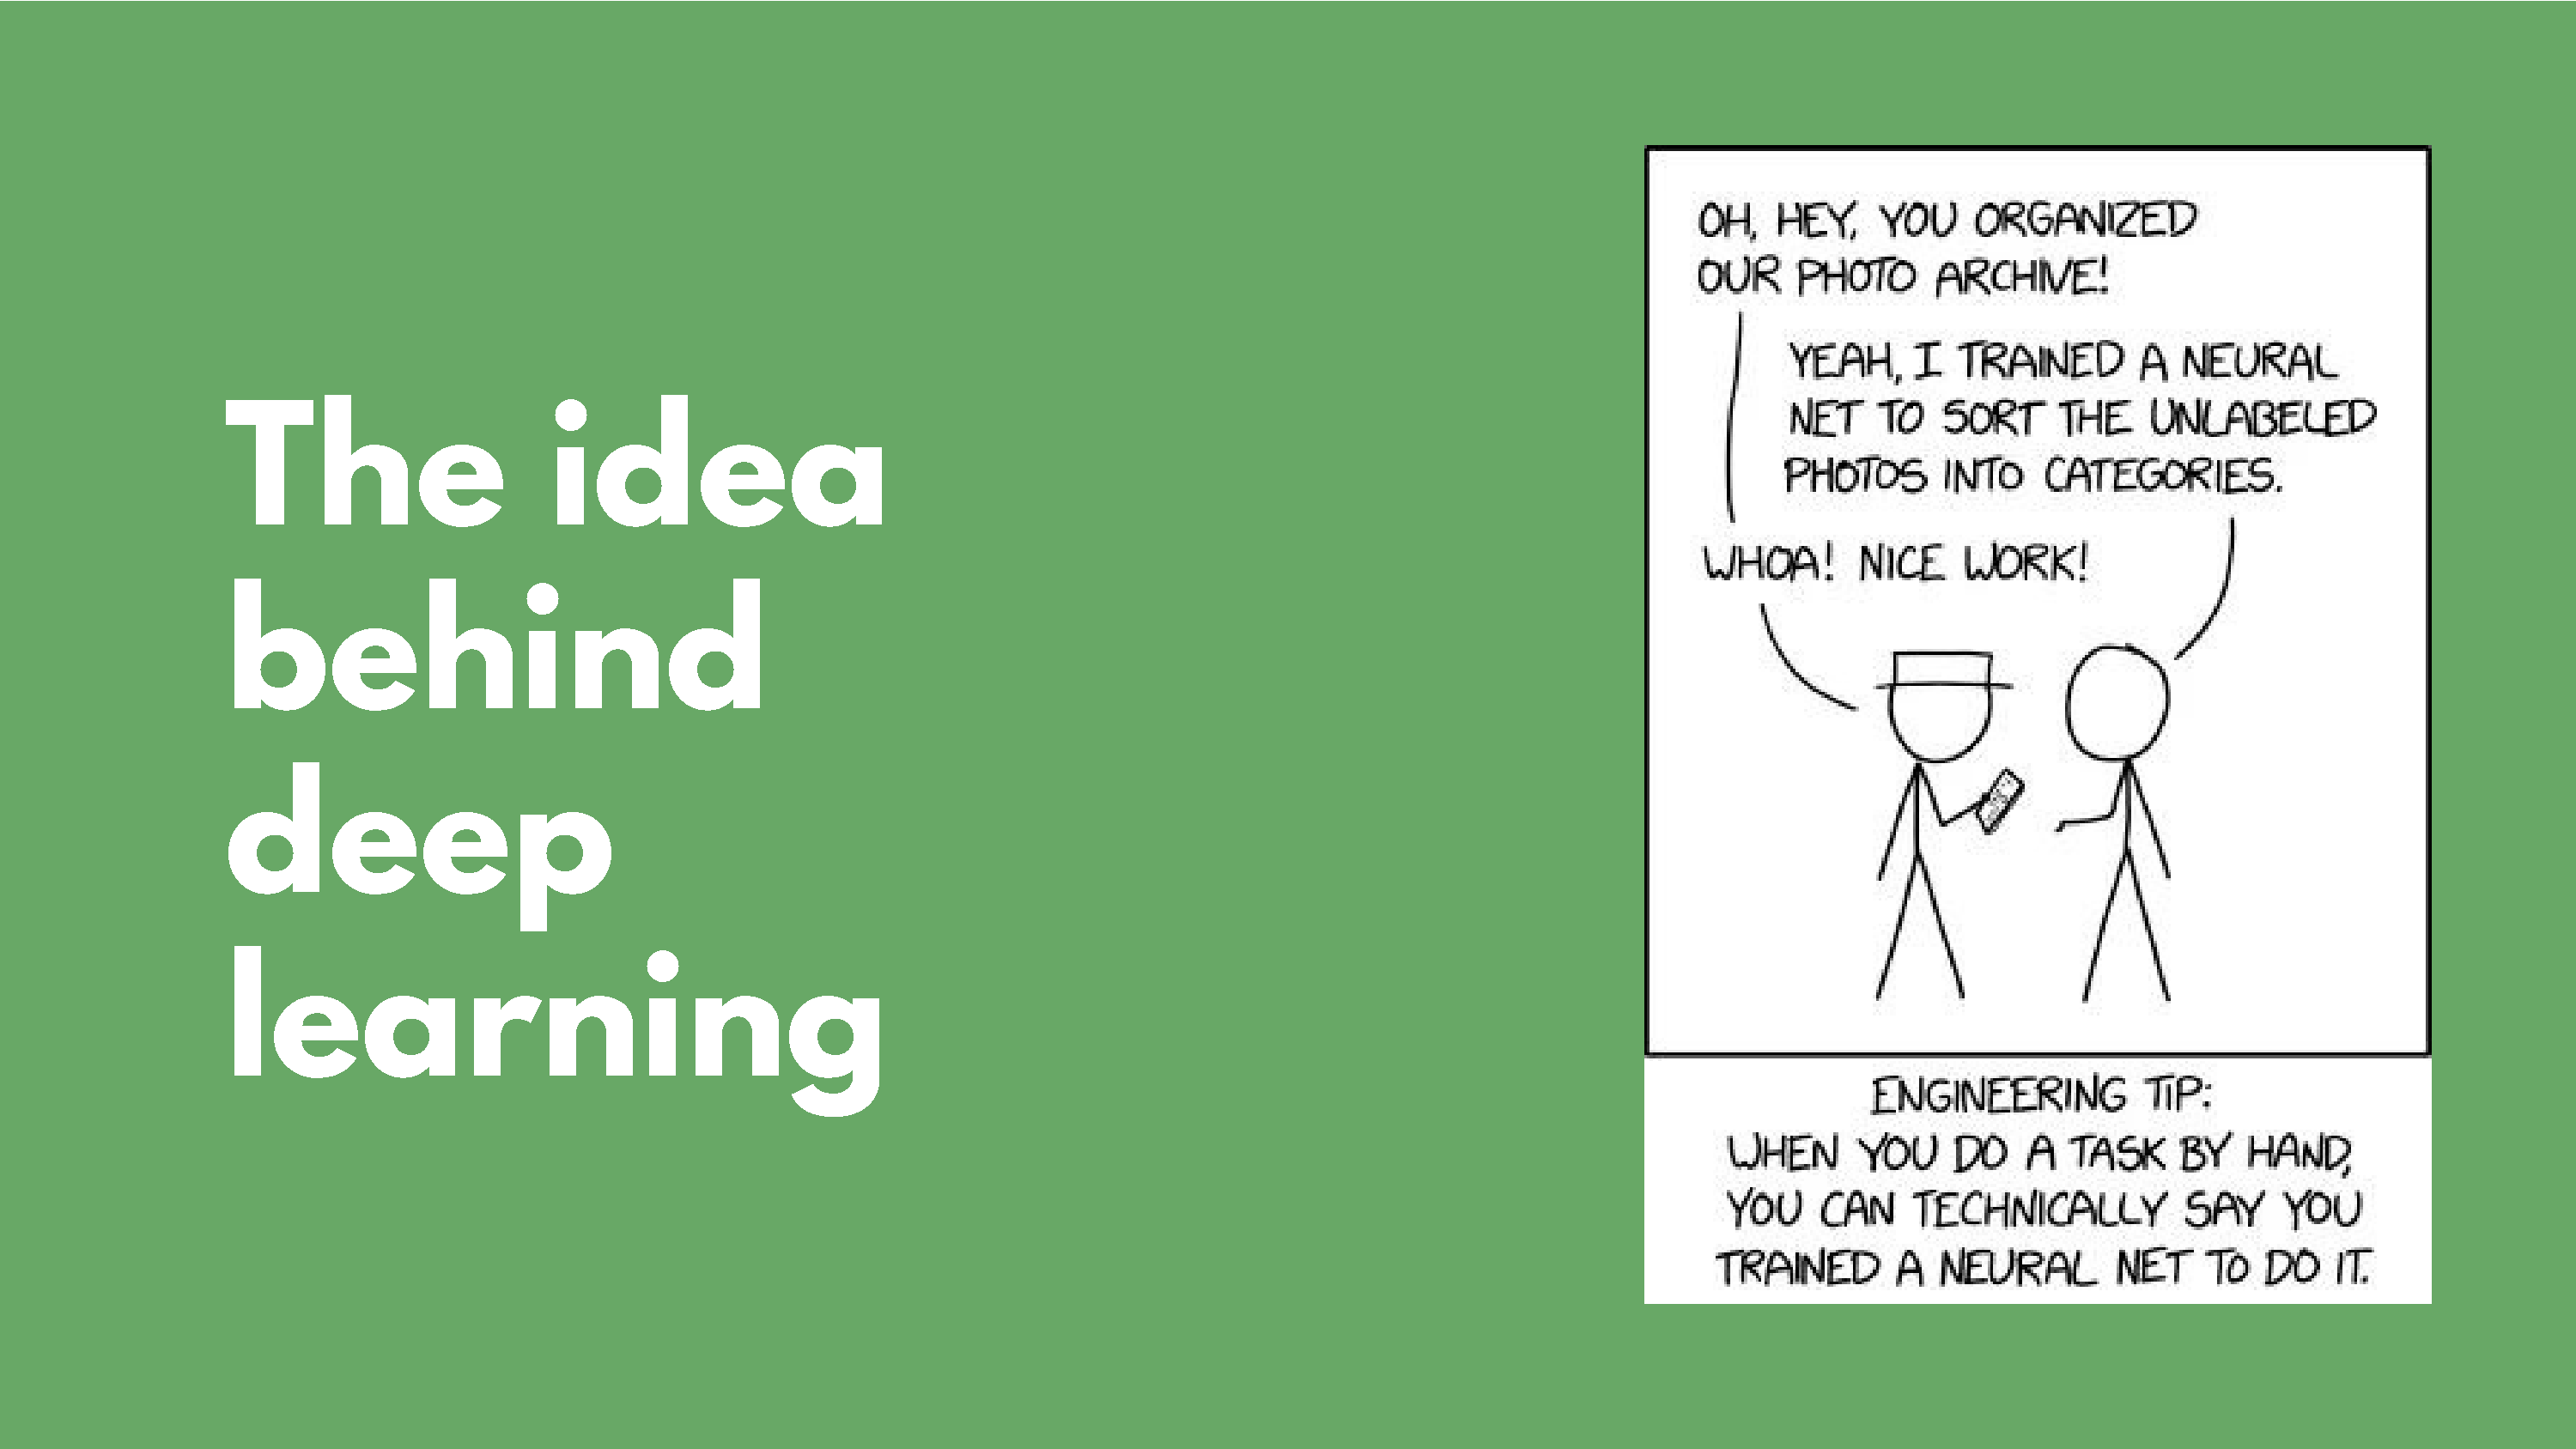
\includegraphics[height=\paperheight,width=\paperwidth]{images/idea_ddepl.pdf}};
  }
  
  \begin{frame}
  \end{frame}
  
  \usebackgroundtemplate{ }
  %edit as needed

\begin{frame}{Ideas behind a neural network}
\begin{enumerate}[$\bullet$]
    \item \textbf{Pattern recognition}: Almost all the problems with traditional Ml lies in proper feature selection. We now take a different approach: We train the machine to learn what the necessary patterns/features are.\pause
    \item \textbf{Inspiration}: For this task we take inspiration from the best pattern recognizing machine that we know:\pause\textbf{ our brains}.\pause
    \item \textbf{Overview}: We make a perceptron, which is essentially the digital analog of a neuron. We connect multiple neurons together(similar to our brain) and look at what pattern and amount of activation leads to best result.
\end{enumerate}
\end{frame}



\begin{frame}{A practical comparison with traditional ML}
    \begin{columns}[T]
    \begin{column}{0.4\textwidth}
      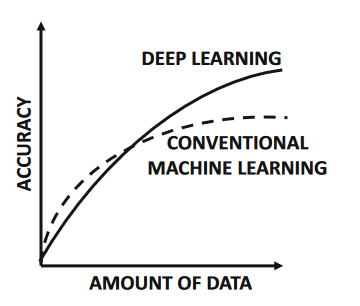
\includegraphics[width=\textwidth]{images/trad vs deep.png}
      \tiny{\textit{Comparision based on amount of data features.\\ Src: Neural Networks and Deep Learning: A Textbook, Charu C. Aggarwal}}
    \end{column}
    \begin{column}{0.6\textwidth}
    \begin{enumerate}[$\bullet$]
    \item Traditional ML models show better prediction when the amount of features involved is small. Features can be individually engineered and interpreted.\pause
    \item Deep learning models are better when data is unstructured or there are a lot of features which need to be considered. With proper construction and training almost any decision boundaries can be learned. 
    \end{enumerate}
    \end{column}
  \end{columns}
\end{frame}

\usebackgroundtemplate{%             declare it
\tikz[overlay,remember picture] \node[opacity=1, at=(current page.center)] {
   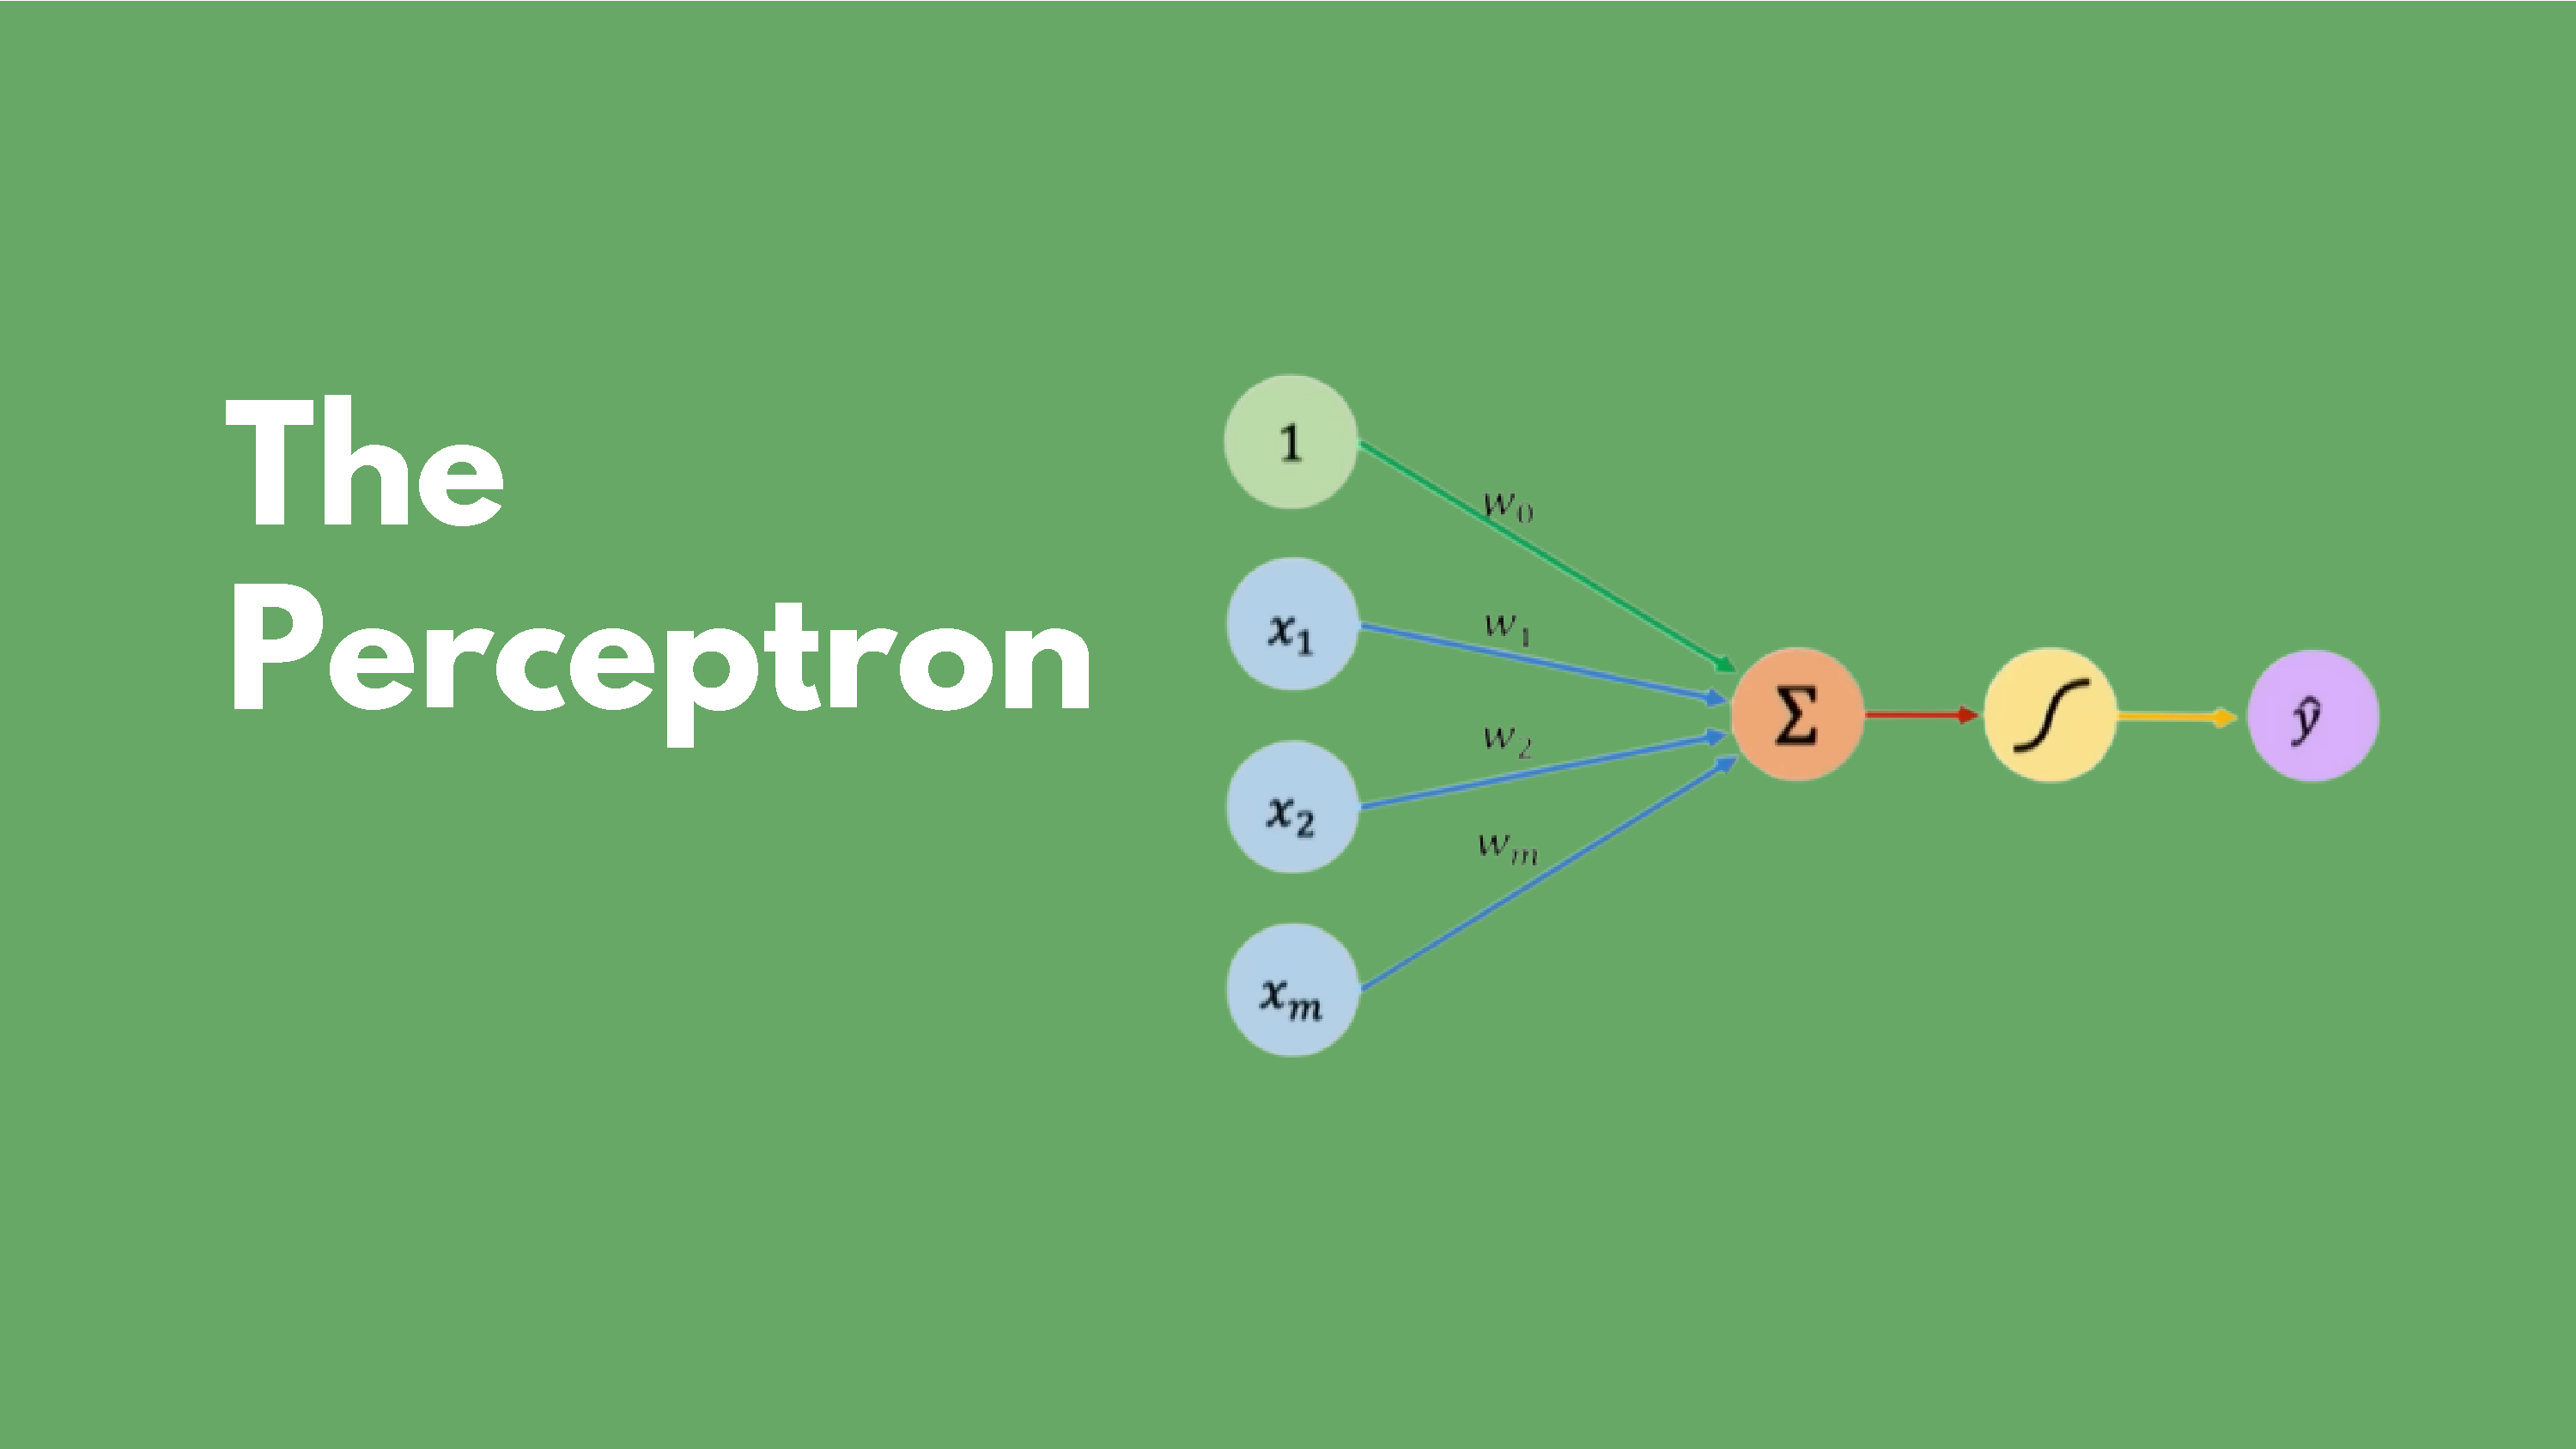
\includegraphics[height=\paperheight,width=\paperwidth]{images/perceptron.pdf}};
}

\begin{frame}
\end{frame}

\usebackgroundtemplate{ }


\begin{frame}{Non-Linearity is the key}
  \begin{columns}[T]
  \begin{column}{0.4\textwidth}
    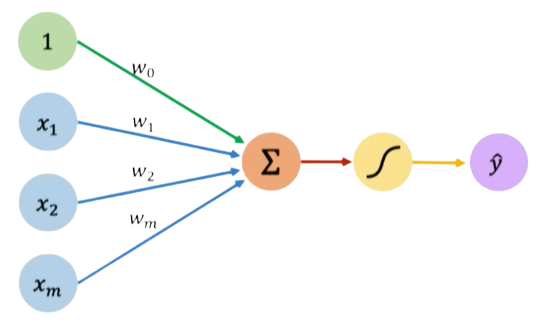
\includegraphics[width=\textwidth]{images/nobg perceptron.png}
    \tiny{\textit{A perceptron\\ Src: MIT Introduction to Deep Learning,6.S191,Lec-1}}
  \end{column}
  \begin{column}{0.6\textwidth}
  \begin{enumerate}[$\bullet$]
  \item The idea behind a perceptron is that a perceptron will give a high value as output when it recognises a certain feature.\pause
  \item Mathematically for an input vector $X$ it outputs $\hat{Y}=\sigma(W^TX+b_0)$ \pause
  \item Multiple perceptrons are wired together(again, much like our brain) to identify richer features.\pause
  \item At the very core, Machine Learning works by constructing proper decision boundaries.\pause
  \item A very simple calculation shows if $\sigma$ is linear then the decision boundary is also linear. It therefore makes sense to use non-linear $\sigma$.
  \end{enumerate}
  \end{column}
\end{columns}
\end{frame}


\begin{frame}{Non-Linearity is the key}
  \begin{columns}[T]
  \begin{column}{0.4\textwidth}
    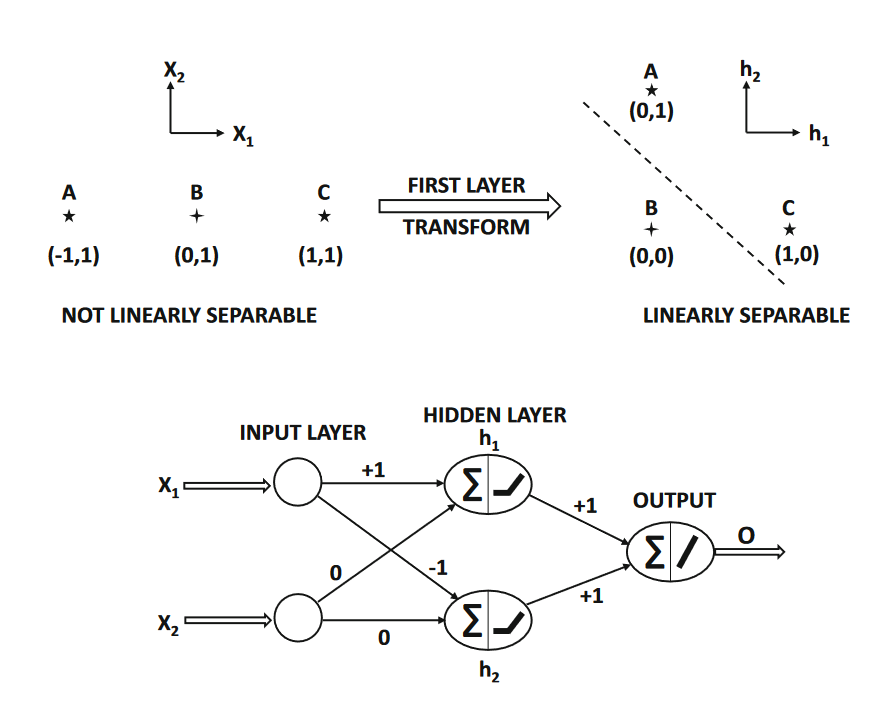
\includegraphics[width=\textwidth]{images/non-linearity.png}
    \tiny{\textit{Non-linearity in action\\ Src: Neural Networks and Deep Learning: A Textbook, Charu C. Aggarwal}}
  \end{column}
  \begin{column}{0.6\textwidth}
  \begin{enumerate}[$\bullet$]
  \item As shown in the figure on left, classes which can't be separated by linear boundaries can be separated by non-linear functions.(Think SVM but the kernals are learned.)\pause
  \item It can be theoretically shown that almost all boundary function can be separated by a 2 layered neural network.
  \end{enumerate}
  \end{column}
\end{columns}
\end{frame}



\begin{frame}{Increasing depth}
  \begin{columns}[T]
  \begin{column}{0.4\textwidth}
    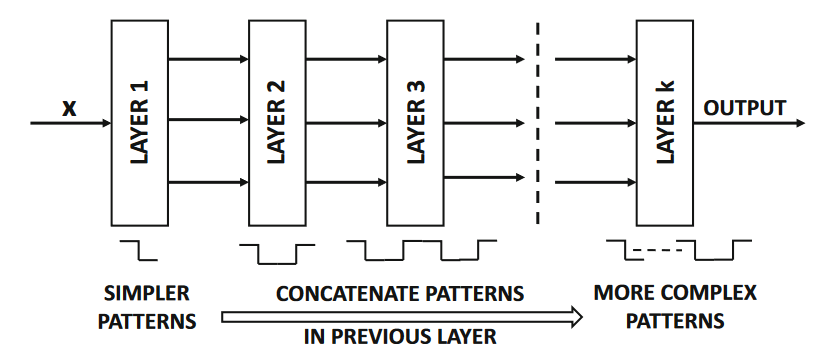
\includegraphics[width=\textwidth]{images/depth.png}
    \tiny{\textit{Why is depth needed\\ Src: Neural Networks and Deep Learning: A Textbook, Charu C. Aggarwal}}
  \end{column}
  \begin{column}{0.6\textwidth}
  \begin{enumerate}[$\bullet$]
  \item While a single hidden layer is enough, making a deep neural network allows us to have more complex decision boundaries with relatively less number of nodes\pause
  \item It should be noted how non-linearity discussed above plays an important role: Irrespective of number of layers, composition of linear functions is linear. On the other hand compositions of non-linear function can lead to richer families of functions. (\textit{Ref: https://www.desmos.com/calculator/m645ggyl2i})
  \end{enumerate}
  \end{column}
\end{columns}
\end{frame}



usebackgroundtemplate{%             declare it
\tikz[overlay,remember picture] \node[opacity=1, at=(current page.center)] {
   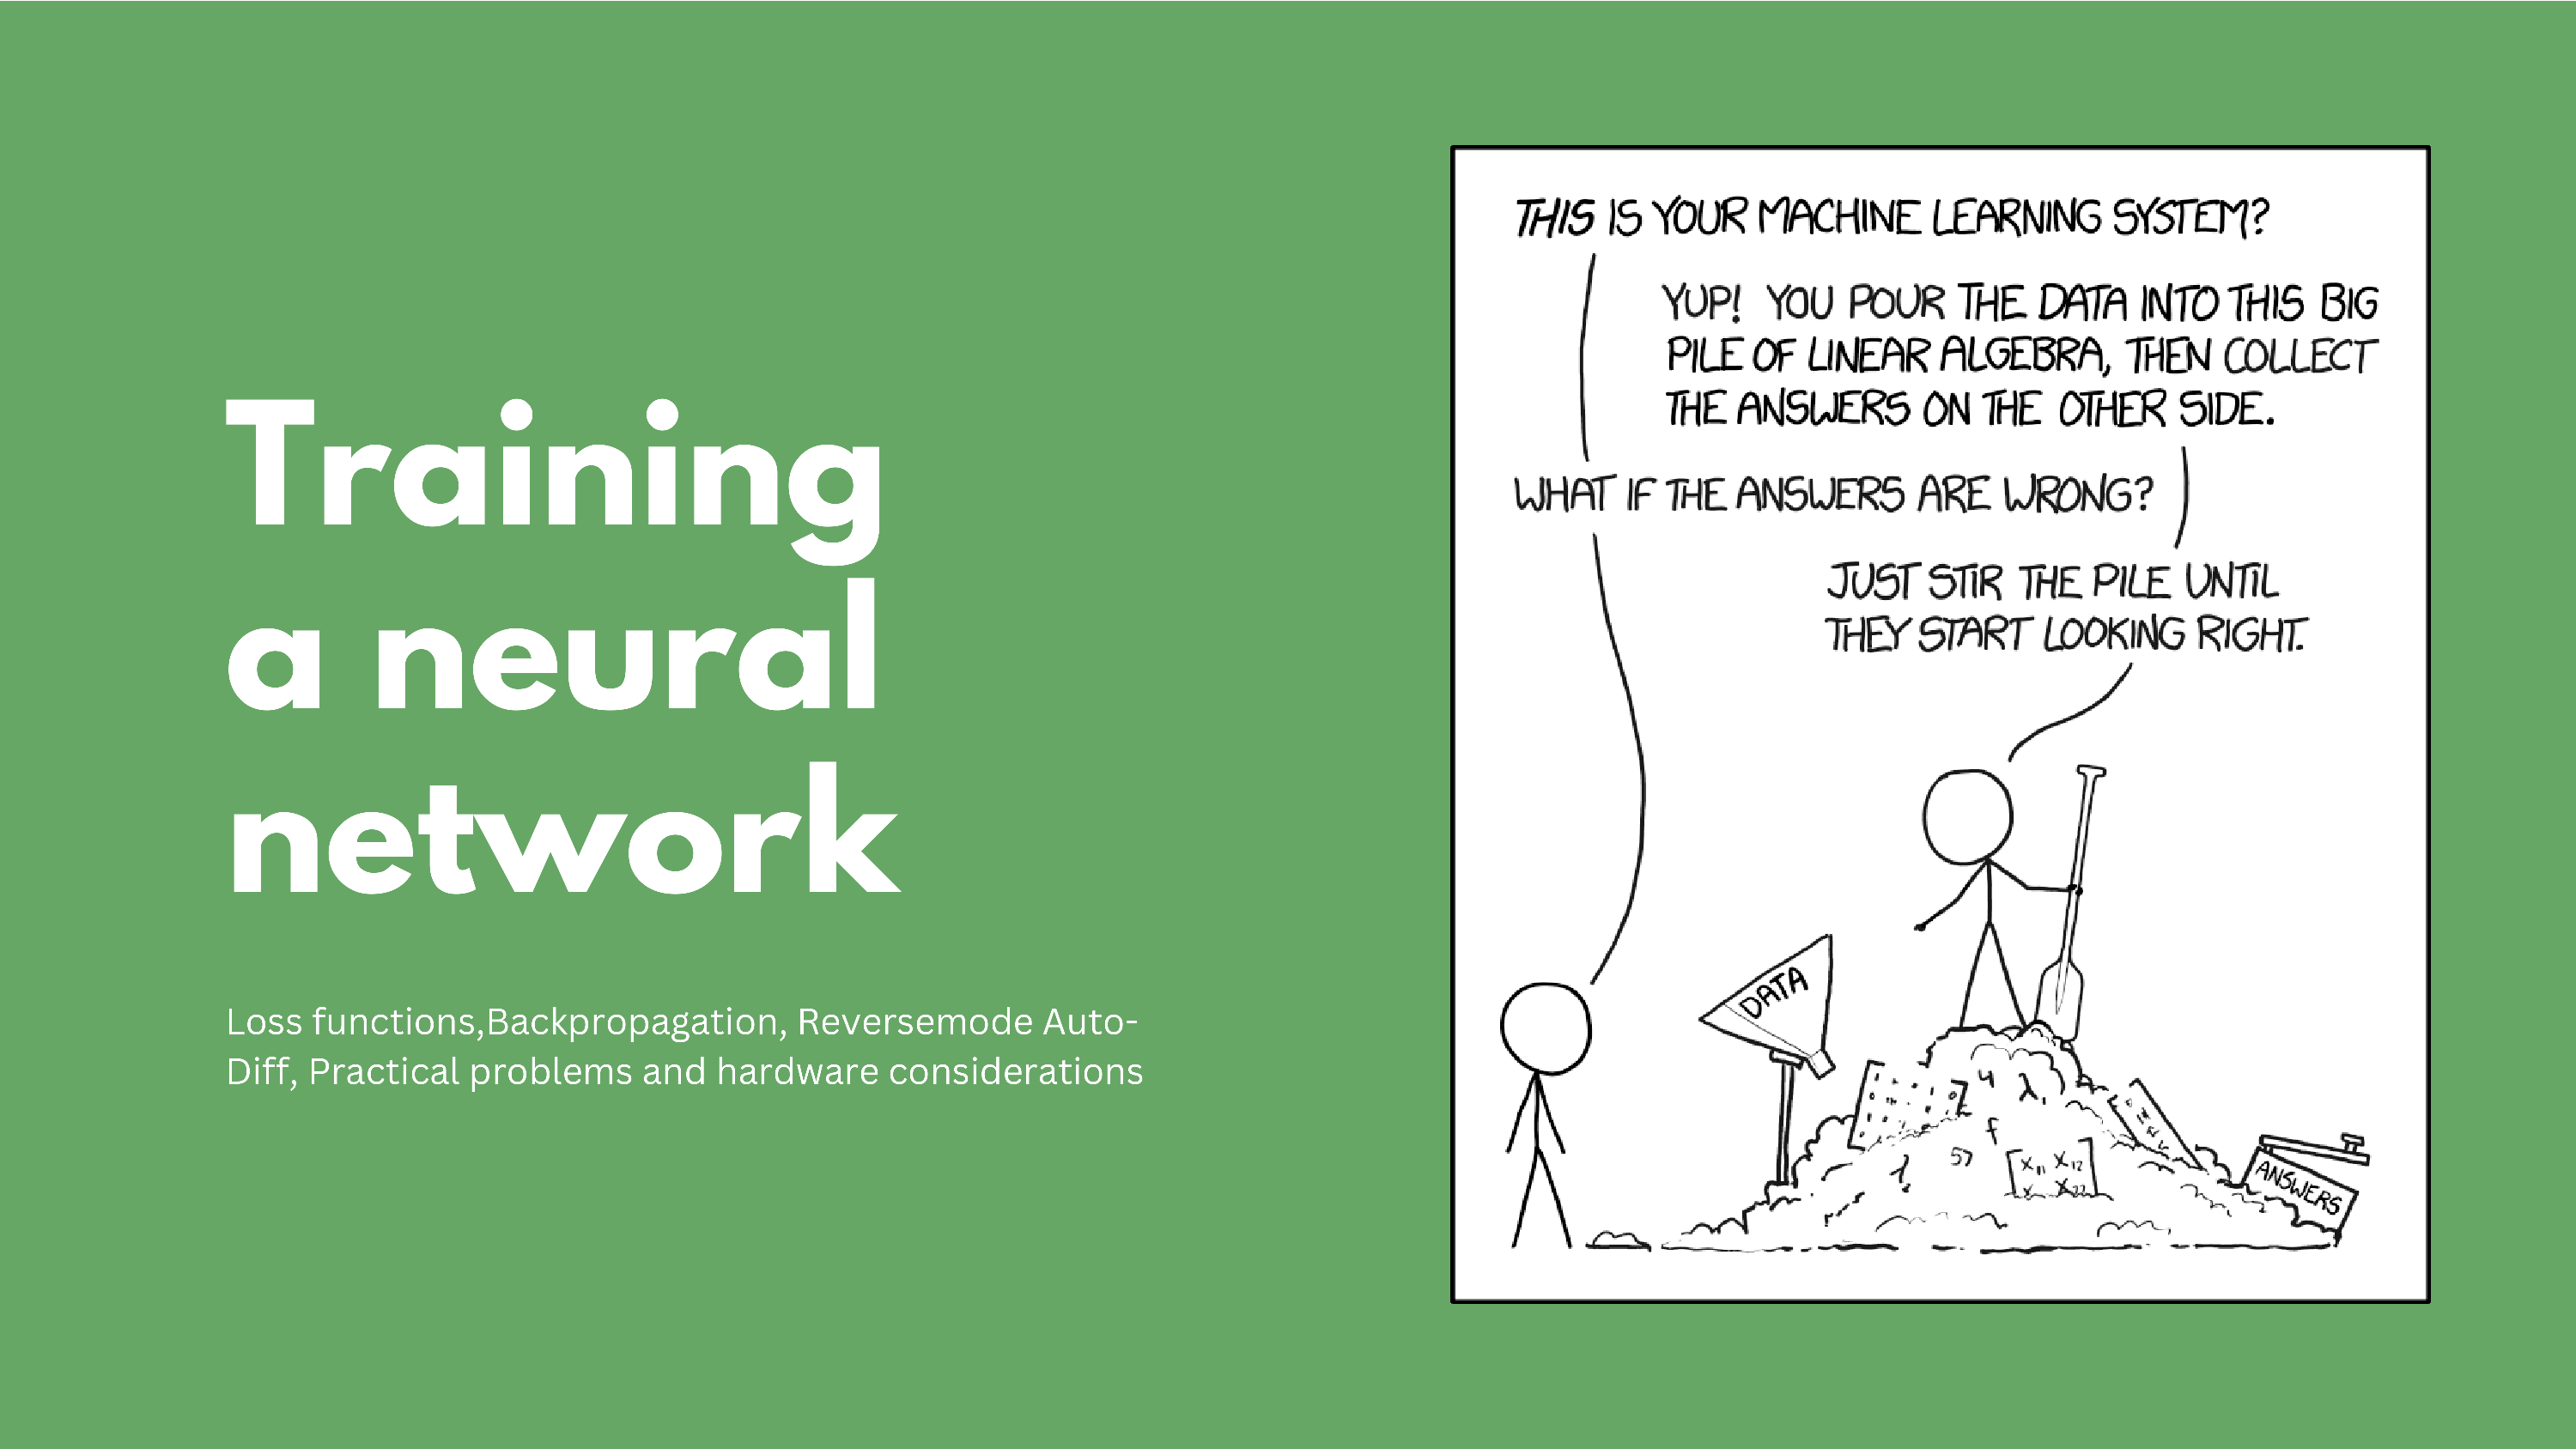
\includegraphics[height=\paperheight,width=\paperwidth]{images/training.pdf}};
}
\begin{frame}
\end{frame}

\usebackgroundtemplate{ }

\begin{frame}{Loss Function}
  \begin{columns}[T]
  \begin{column}{0.4\textwidth}
    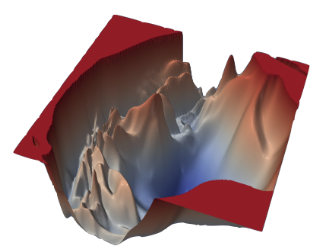
\includegraphics[width=\textwidth]{images/resnet110-noskip-loss.png}
    \tiny{\textit{A slice of the loss landscape of resnet-110 with no skip connections\\ Src: Visualizing the Loss Landscape of Neural Nets, Hao Li, Zheng Xu, Gavin Taylor, Christoph Studer, Tom Goldstein}}
  \end{column}
  \begin{column}{0.6\textwidth}
  \begin{enumerate}[$\bullet$]
  \item We wish to calculate weights $w_i,1\leq i\leq n$ so that the predicted values $\hat{Y}$ are as close as possible(to an extent) to the actual values $Y$.\pause To do this we try to minimize a loss function $\mathcal{L}(\{\hat Y_i\},\{Y_i\})$\pause
  \item Common choices of $\mathcal L$ include MSE for continuous variables and cross-loss entropy for categorical variables.
  \end{enumerate}
  \end{column}
\end{columns}
\end{frame}


\begin{frame}{Gradient descent}
  \begin{columns}[T]
  \begin{column}{0.4\textwidth}
    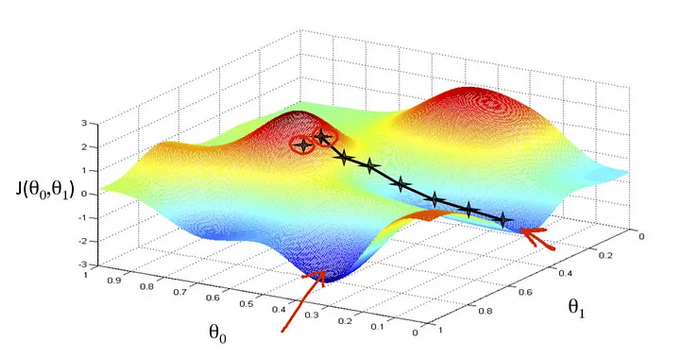
\includegraphics[width=\textwidth]{images/grad-desc.png}
    \tiny{\textit{Gradient descent\\ Src: https://towardsdatascience.com/an-intuitive-explanation-of-gradient-descent-83adf68c9c33}}
  \end{column}
  \begin{column}{0.6\textwidth}
  \begin{enumerate}[$\bullet$]
  \item To find the correct set of weights, we use a greedy approach. We check the surrounding landscape of the weight(i.e. calculate the gradient) and take a step in the direction which leads to maximum decrease in $\mathcal L$. Mathematically, we have:
  $$w_i=wi-\eta \frac{\partial \mathcal L}{\partial w_i}$$\pause
  \item $\eta$ is known as the learning rate.
  \end{enumerate}
  \end{column}
\end{columns}
\end{frame}


\begin{frame}{Learning Rate}
  \begin{columns}[T]
  \begin{column}{0.4\textwidth}
    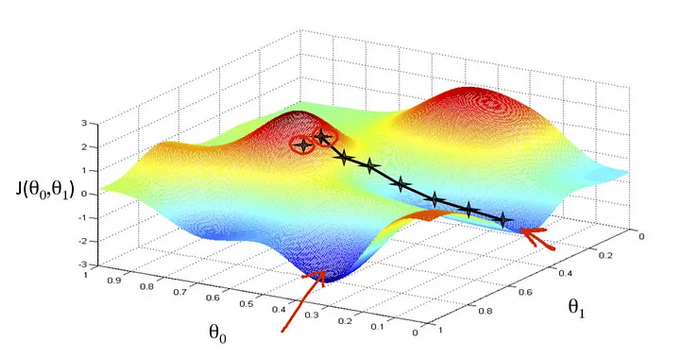
\includegraphics[width=\textwidth]{images/grad-desc.png}
    \tiny{\textit{Gradient descent\\ Src: https://towardsdatascience.com/an-intuitive-explanation-of-gradient-descent-83adf68c9c33}}
  \end{column}
  \begin{column}{0.6\textwidth}
  \begin{enumerate}[$\bullet$]
  \item Fixing $\eta$ is quite tricky.\pause
  \item If $\eta$ is small we get stuck at local minima\pause
  \item If $\eta$ is large we overshoot our targets and never converge.
  \item The best way to do things is to use a adaptive learn rate. Some methods(parametric, non-parametric and hybrid are discussed later, once we cover backpropagation)
  \end{enumerate}
  \end{column}
\end{columns}
\end{frame}


\begin{frame}{Backpropagation}
  Consider an acyclic directed graph. 
  \begin{enumerate}[$\bullet$]
  \item We want to calculate the partial derivative of a node with respect to the other.\pause
  \item The way to do this is to use the chain rule\pause
  \item When we use the chain rule, we sum the partial derivative along all the paths joining the two nodes
  \item It is easy to see that the computation needed explodes as the depth increases
  \item The way to navigate this problem is to use dynamic programming.
  \end{enumerate}
\end{frame}
